%\documentclass{aa}
\documentclass[referee]{aa}

\usepackage{color}

%\bibpunct{(}{)}{;}{a}{}{,};
\usepackage{amsmath}
\usepackage{natbib}
\usepackage{graphicx}
%------------------------------------------------------------------------
%Added by language editor to facilitate margin notes.
%------------------------------------------------------------------------
%\usepackage{marginnote}
\usepackage{color}
\setlength{\marginparwidth}{40mm}
\setlength{\marginparsep}{5mm}
\newcommand{\aamarginnote}[1]{{\boldmath$\color{red}\bigvee$}
\marginpar{\baselineskip3ex{\color{red}#1}}}
\newcommand{\mvn}[1]{{\color{red}Michiel:  #1}}
\newcommand{\im}[1]{{\color{blue}Ivan:  #1}}
%------------------------------------------------------------------------
\begin{document}

   \title{Line response functions in non-local thermodynamic equilibrium}

   \subtitle{Isotropic case}

   \author{I. Mili\'{c}\inst{1}
   \and
   M. van Noort\inst{1}}
   
   \institute{Max-Planck-Institut f\"{u}r Sonnersystemforschung, Justus-von-Liebig-Weg 3, 37077 G\"{o}ttingen, Germany\\
   \email{milic@mps.mpg.de; vannoort@mps.mpg.de}}
         %\and
         %Astronomical observatory Belgrade, Volgina 7, 11060 Belgrade, Serbia\\
          %   }

   \date{}
   \titlerunning{Response functions in NLTE}
   \authorrunning{I. Mili\'{c} \& M. van Noort}

% \abstract{}{}{}{}{} % 5 {} token are mandatory

  \abstract
  % context heading (optional)
   {Response functions provide us with a quantitative measure of sensitivity of the emergent spectrum to perturbations in the solar atmosphere and are thus the method of choice for interpretation of spectropolarimetric observations. For the lines formed in the solar chromosphere, it is necessary to compute these responses taking into account non-local thermodynamic equilibrium (NLTE) effects.}  
  % aims heading (mandatory)
  {We show how to analytically compute the response of the level populations in NLTE to a change of a given physical quantity at a given depth in the atmosphere. These responses are then used to compute opacity and emissivity responses, which are then propagated to obtain the response of the emergent intensity.}
   % methods heading (mandatory)
   {Our method is based on the derivative of the rate equations, where we explicitly incorporate spatial coupling in the radiative rate terms. After considering and collecting all inter-dependencies, the problem reduces to a linear system of equations with a dimension equal to the product of the number of spatial points and the number of energy levels.}
  % results heading (mandatory)
   {We compare analytically computed response functions with ones obtained using a finite difference approach and find very good agreement. In addition, a more accurate way of propagating opacity and emissivity perturbations through the numerical solution of the radiative transfer equation was developed.} 
  % conclusions heading (optional), leave it empty if necessary
   {This method allows for the fast evaluation of the response of the emergent spectrum to perturbations of a given quantity at a given depth, and thus is a significant step towards more efficient NLTE inversions.}
 
   \keywords{Line: formation; Radiative transfer, Scattering}

   \maketitle

%___________________________________________________________________________________

\section{Introduction}

Response functions of spectral lines \citep{Mein71, Beckers75, Landi77} describe the sensitivity of an emergent Stokes spectrum to the perturbations of physical parameters as a function of depth in the atmosphere \citep[for a detailed study of the possible diagnostics see][]{RFs94}. Although they are useful in forward modeling, to propose and analyze various diagnostics \citep[e.g.][]{Han06}, their main strength and application is in derivative-based spectral line fitting \citep[in solar physics widely known as ``inversion'', see for example][]{SIR}. Given the perturbation of an atmospheric parameter (temperature, velocity, magnetic field, etc.), the computation of the response function in practice reduces to the computation of the responses (derivatives with respect to atmospheric parameters) of opacity and emissivity and then propagating these responses using the formal solution of radiative transfer equation. It is intuitively clear that finding the responses of opacity and emissivity requires the responses of the atomic and molecular number densities as well as responses of the populations of individual levels. 
%We will try to make this dependence clear and explicit in the remainder of the paper.

In the approximation of local thermodynamical equilibrium (LTE), computing responses of level populations is relatively straightforward \citep[e.g.][]{SIR, dtibook}, as all the relevant number densities depend only on local quantities. In addition, level populations and their response can be computed analytically, using Saha-Boltzmann equation. LTE is a good approximation for the spectral lines formed deep in the photosphere, where transitions between the levels are dominated by collisions. However, for lines which are formed in the upper photosphere and the chromosphere (e.g. H$\alpha$, Ca\,II infrared triplet, Ca\,II H\&K, Mg h\&k lines, to name just a few), this approximation is far from valid as the transition rates are dominated by the radiation field. This introduces both spatial and nonlinear coupling between the level populations, resulting in a so-called NLTE problem. The solution of such problems is extensively discussed in the literature and probably the best reference is a classical monograph by \citet{Mihalasbook} \citep[or a recent re-issue by][]{SAbook2014}. For polarized radiation, however, there are wealth of unsolved and interesting problems, a detailed and comprehensive introduction is given in \citet{LL04}.

The response of a NLTE problem to atmospheric changes, however, has not been studied in great detail. The first attempt, by \citet{HectorI}, was based on the so called FDC (fixed departure coefficients) approximation, which essentially computes the NLTE response functions by scaling the LTE ones with the departure coefficients (the departure coefficient is the ratio of the level population in NLTE to the one in LTE). In that paper, the authors find that this is a rather crude approximation and resort to computing the response functions numerically (i.e. using finite differences) instead. In the papers of \citet{Hector_halpha} and \citet{Han06}, response functions are computed numerically. Also, in the NLTE inversion code NICOLE \citep{NICOLE}, responses, and thus the $\chi^2$ derivatives to model parameters, are computed in a numerical way.

In this paper we demonstrate how the response functions of the level populations to atmospheric quantities can be computed in an analytical way, at a significantly reduced computational cost as compared to finite differencing, from which it is straightforward to compute the response functions of the opacity and emissivity. Given the perturbations of opacity and emissivity, we show how to compute very precisely the resulting perturbations of the intensity throughout the atmosphere. In Section 2 we outline the method for analytical computation of NLTE functions and show the explicit derivation for a case of pure line transfer. In Section 3 we compare analytically computed response functions with ones computed using finite differences and discuss the discrepancies. Finally we conclude by discussing possible applications of our approach and future steps. 

\section{Response functions}
\label{concept}

In the following, we will assume that the emergent radiation is formed in a plane-parallel atmosphere represented by a discrete set of points in a single dimension (1D), at which the values of atmospheric parameters are given. The relevant atmospheric parameters for the formation of spectral lines are: temperature, pressure, line-of-sight 	velocity, microturbulent velocity and the magnetic field. Given the values of these parameters, we can obtain the opacity and the emissivity of the medium at each spatial and spectral point, and in each direction. These then enter the radiative transfer equation (RTE), which in the 1D axisymmetric, time-independent, polarization-free case reads:
\begin{equation}
 \mu \frac{dI(z,\mu,\lambda)}{dz} = -\chi(z,\mu,\lambda) I(z,\mu,\lambda) + \eta(z,\mu,\lambda),
 \label{rte}
\end{equation}
where $z$ is the geometrical coordinate along the surface normal, $\mu = \cos \theta$, where $\theta$ is the angle with respect to the surface normal, and $\chi$ and $\eta$ are the unpolarized (i.e. scalar) opacity and emissivity respectively. Given the boundary conditions, the solution of the radiative transfer equation then yields the emergent intensity spectrum, which is to be compared with, or fitted to the observed one. Note that the emergent intensity depends on the opacity and emissivity throughout the whole atmosphere (i.e. the solution is non-local). This non-locallity is explicitly seen from the so called formal solution of radiative transfer equation:
\begin{equation}
 I_0(\mu,\lambda) = \int_0^{\infty} S(\tau_{\lambda},\mu,\lambda) e^{-\tau_{\lambda}} d\tau_{\lambda} / \mu
\end{equation}
where $S=\frac{\eta(\tau_{\lambda},\mu,\lambda)}{\chi(\tau_{\lambda},\mu,\lambda)}$ is the source function and $\tau_{\lambda}$ is monochromatic optical depth defined by $d\tau_{\lambda} = -\chi(z,\mu,\lambda)dz$.

We define the response function of the emergent intensity to the change of a given atmospheric quantity $q$ at depth point $k$ in the following way:
\begin{equation}
 R_{q_k} \equiv \frac{\partial I_0(\mu,\lambda)}{\partial q_k},
\end{equation}
which is readily expressed in terms of the derivatives of the emergent intensity to opacity and emissivity, 
\begin{align}
 \frac{\partial I_0(\mu,\lambda)}{\partial q_k} = & \sum_l^{N_D} \frac{\partial I_0(\mu,\lambda)}{\partial \chi_l(\mu,\lambda)} \frac{\partial \chi_l(\mu,\lambda)}{\partial q_k} \nonumber \\
 + & \sum_l^{N_D} \frac{\partial I_0(\mu,\lambda)}{\partial \eta_l(\mu,\lambda)} \frac{\partial \eta_l(\mu,\lambda)}{\partial q_k},
 \label{resp1}
\end{align}
where $N_D$ is number of depth points in the atmosphere. The summation over $l$, the numerical equivalent of integration over the entire atmosphere, stems from the observation that a perturbation $q_k$ in point $k$ in general changes the opacity and emissivity not only in point $k$, but in the whole atmosphere. In general, $\frac{\partial I_0(\mu,\lambda)}{\partial \chi_l(\mu,\lambda)}$ and $\frac{\partial I_0(\mu,\lambda)}{\partial \eta_l(\mu,\lambda)}$ depend on the exact scheme used to solve the RTE, and we discuss this computation in more detail in appendix\,\ref{Appendix_A}. For the time being, however, we will assume that we are able to compute $\frac{\partial I_0}{\partial \chi_l}$ and $\frac{\partial I_0}{\partial \eta_l}$ in some way (we are omitting angle and wavelength dependence, which should be clear from the context).

To evaluate (\ref{resp1}), we require the derivatives of the opacity and the emissivity everywhere with respect to quantity $q_k$. For the sake of simplicity, we restrict the discussion here to line processes only, and relax this assumption later. In the case of pure line transfer, we have
\begin{align}
 \chi_l(\mu,\lambda) = \frac{h\nu}{4\pi}(n_{l,j} B_{ji} - n_{l,i}B_{ij}) \phi^{ij}_l(\mu,\lambda),
\end{align}
where $i$ and $j$ are the indices of the upper and lower levels of each transition, $n_{l,i}$ denotes the number density of atoms in state $i$ at spatial point $l$, $B_{ji}$ and $B_{ij}$ are Einstein coefficients of absorption and stimulated emission, respectively and $\phi^{ij}_l(\lambda)$ is the line absorption profile. Similarly:
\begin{align}
 \eta_l(\mu,\lambda) = \frac{h\nu}{4\pi}n_{l,i}A_{ij} \phi^{ij}_l(\mu,\lambda) 
\end{align}
where $A_{ij}$ is Einstein coefficient of spontaneous emission. Here we have assumed complete frequency redistribution (CRD), which is a good approximation for most spectral lines of interest, with the exception of very strong lines, that are formed very high in the atmosphere. Even for those lines, however, CRD usually describes the line core very well.

The derivative of the opacity with respect to $q_k$ is then:
\begin{align}
  \frac{\partial \chi_l(\mu,\lambda)}{\partial q_k} = & \frac{h\nu}{4\pi}(n_{l,j} B_{ji} - n_{l,i}B_{ij}) \frac{\partial\phi^{ij}_l(\mu,\lambda)}{\partial q_k} \nonumber \\
 + & \frac{h\nu}{4\pi}(\frac{\partial n_{l,j} B_{ji}}{\partial q_k} - \frac{\partial n_{l,i}B_{ij}}{\partial q_k}) \phi^{ij}_l(\mu,\lambda).
 \label{chi_derivative}
\end{align}
A similar expression can be written for the derivative of the emissivity. We thus see that the derivative (response) of the opacity/emissivity can be expressed through the derivatives of the level populations and the derivative of local absorption profile. The latter is determined by the temperature, microturbulent velocity and the number density of the collisional partners (neutral hydrogen, electrons, etc.). 

Although in the general problem, we can find the NLTE responses of electron density simultaneously with all other atomic populations, if we assume that the electron density is either constant or that its response can be approximated by the LTE response, the calculation of the derivative of the absorption profile becomes strictly local, that is:
\begin{equation}
 \frac{\partial\phi^{ij}_l(\mu,\lambda)}{\partial q_k} = \delta_{lk} \frac{\partial\phi^{ij}_k(\mu,\lambda)}{\partial q_k},
\end{equation}
so that the only remaining quantities to be computed are the derivatives of the level populations. Because the approximation of LTE does not hold, this is the most complicated part of the computation.

\subsection{Responses of populations in NLTE}
\label{nlte_lvls}

Where the approximation of LTE is accurate, the level populations are determined only by local quantities, and can be obtained with relative ease. However, if the density is sufficiently low, the approximation of LTE is not valid, and the level populations are determined both by the local temperature and by the (non-local) radiation field. Under such so-called non-LTE (NLTE) conditions, the level populations are goverend by the population evolution equation which, for the population of level $i$ at depth point $l$, reads:
\begin{equation}
 \frac{d n_{l,i}}{d t} = \sum_j (n_{l,j} T_{l,ji} - n_{l,i} T_{l,ij}).
\end{equation}
This is a non-linear and non-local set of coupled differential equations, which is notoriously difficult to solve. However, if the conditions can be assumed stationary, $\frac{d n_{l,i}}{d t} = 0$, then we can solve the considerably friendlier statistical equilibrium equation
\begin{equation}
 \sum_j (n_{l,j} T_{l,ji} - n_{l,i} T_{l,ij}) = 0
 \label{SE}
\end{equation}
instead. Here $T_{ij}$ is total rate of transitions from level $i$ to level $j$. Generally, $T_{ij} = C_{ij} + R_{ij}$ where $C$ stands for collisional and $R$ for radiative transitions.

Deep in the photosphere, the density is so high that collisional rates dominate over the radiative ones and thus the approximation of LTE may be used. However, the situation is reversed in the chromosphere, with radiative transitions dominating over collisions. This means that the populations of the energy levels are no longer determined only by the temperature, but also by the radiation field, and, since the radiation field in turn depends on the emissivity and opacity, the radiation field thus effectively depends on itself. Many spectral lines are very optically thin in this region and this effect can be safely neglected, but for some spectral lines that are sufficiently strong to be still optically thick there, the populations must be calculated using (\ref{SE}), self-consistently with the radiation field using (\ref{rte}). 

At least from the theoretical point of view, this problem can be considered ``solved'' mostly thanks to the application of so called ``Accelerated Lambda Iteration'' methods \citep[for an insightful review see][]{Hubeny03}.  Here, we want to go one step further and compute not only the populations but also their responses (derivatives). For brevity, we use following notation:
\begin{equation}
 {\mathcal R}_{lik} \equiv \frac{\partial n_{l,i}}{\partial q_k}
\end{equation}
and refer to it as ``response functions of level populations.'' To compute them, we start by differentiating Eq.\,\ref{SE} with respect to $q_k$:
\begin{equation}
 \sum_j \left ({\mathcal R}_{ljk} T_{l,ji} - {\mathcal R}_{lik} T_{l,ij} + n_{lj} \frac{\partial T_{l,ji}}{\partial q_k} - n_{li} \frac{\partial T_{l,ji}}{\partial q_k} \right ) = 0.
 \label{rateder1}
\end{equation}
System in Eq.\,\ref{SE} is undetermined, so the statistical equilibrium equation for one of the levels is usually replaced with:
\begin{equation}
 \sum_j n_{lj} = N_l,
\end{equation}
which, after taking the derivative becomes:
\begin{equation}
 \sum_j {\mathcal R}_{ljk} = \frac{\partial N_l}{\partial q_k}.
\end{equation}
Where $N_l$ is the total number density of species in question. For the simplicity's sake we will assume that this derivative is strictly local and that it can be computed directly from the equations of chemical equilibrium. To solve Eq.\,\ref{rateder1} for $\mathcal{R}_{lik}$, we need the derivative of the rates:
\begin{equation}
\frac{\partial T_{l,ji}}{\partial q_k} = \frac{\partial C_{l,ji}}{\partial q_k} + \frac{\partial R_{l,ji}}{\partial q_k}.
\label{rateder2}
\end{equation}
If we neglect the radiative rates both in Eq.\,\ref{SE} and Eq.\,\ref{rateder1} and solve for populations and population responses, we end up with LTE values, however, in this specific case, it is actually easier to find level populations, as well as their responses, directly from the Saha-Boltzmann equations \citep[see, e.g.][]{SIR}. 

If we account for the radiative rates in Eq.\,\ref{SE}, but keep only the collisional rates (and their derivatives) in Eq.\,\ref{rateder1}, we arrive at the FDC (fixed departure coefficients) approximation of \citet{HectorI}, that uses the approximation
\begin{equation}
{\mathcal R}_{lik} = b_{l,i}  {\mathcal R}^*_{lik}
\end{equation}
for the population responses, where ${\mathcal R}^*_{lik}$ denotes the LTE population response function and $b_{l,i}$ is the so-called NLTE departure coefficient of each level. Since the dependence of the departure coefficient on $q_k$ is not taken into account, the non-local spatial coupling is not present, and the responses obtained in this way are therefore strictly local. While this makes the computations much easier, it does not account for the most significant NLTE effect, that of the non-locality, which is usually most pronounced in the upper, more dilute layers of the atmosphere, and becomes more important the finer the spatial grid is. This is probably why \citet{HectorI} find poor agreement between the FDC approximation and numerically computed responses in the upper layers of their atmospheres.

Clearly, a fully consistent approach needs to account not only for the correct radiative rates, but also for the response of those radiative rates.

\subsection{Derivative of radiative rates}
\label{radiative_rates}

The radiative rates we are interested in (bound-bound and bound-free ones) are functionals of the specific intensity, and have the following form:
\begin{equation}
 R_{l,ji} \propto \int_0^{\infty} \int_{-1}^{1} \Psi_{l,ij} I_l{\mu,\lambda}\,d\mu d\lambda,
\end{equation}
where $\Psi_{l,ij}$ is some weighting function (e.g. the profile function in the case of pure line transfer), and $k$. The derivative of the radiative rates then becomes: 
\begin{align}
 \frac{\partial R_{l,ji}}{\partial q_k} \propto \int_0^{\infty} \int_{-1}^{1} & \left [ \frac{\partial\Psi_{l,ij}}{\partial q_k} I_l{\mu,\lambda} + \Psi_{l,ij} \frac{\partial I_l{\mu,\lambda}}{\partial q_k} \right ] \nonumber \\
 & \times d\mu d\lambda.
\end{align}
Further expanding the derivative of the specific intensity, in a similar fashion to Eq.\,\ref{resp1}, we get, omitting dependencies, which should be clear from the context:
\begin{equation}
 \frac{\partial I_l}{\partial q_k} = \sum_{l'} \left[ \frac{\partial I_l}{\partial \chi_{l'}} \frac{\partial\chi_{l'}}{\partial q_k} + \frac{\partial I_l}{\partial \eta_{l'}} \frac{\partial\eta_{l'}}{\partial q_k} \right ].
\end{equation}
Opacity and emissivity depend on all the populations of the relevant species, but also explicitly on the atmospheric parameters:
\begin{equation}
\frac{\partial\chi_{l'}}{\partial q_k} = \frac{\partial\chi_{l'}}{\partial q_k}_{\rm{explicit}} + \sum_i \frac{\partial\chi_{l'}}{\partial n_{l',i}} \frac{\partial n_{l',i}}{\partial q_k},
\label{chi_der}
\end{equation}
where the summation over $i$ takes into account all the relevant energy levels of all the species. A similar equation to Eq.\,\ref{chi_der} can be written for emissivity. Starting from Eq.\,\ref{chi_der} and substituting back all the way to the Eq.\,\ref{rateder1}, we end up with a linear system which couples all points in the atmosphere (because of the radiative transfer), and all the atomic level populations (because of their influence on opacity and emissivity). Below we give an explicit derivation for the case of pure line transfer and in \ref{CaII} we treat the atomic model which also involves radiative bound-free and free-bound rates.

For pure line transfer, the radiative transition rates from bound level $i$ to bound level $j$, have the following form:
\begin{equation}
 R_{l,ij} = A_{ij} + B_{ij} J_{l,ij},
\end{equation}
where $A_{ij} \equiv 0$ when $i<j$ and $J_{l,ij}$ is the so called scattering integral for the transition $i\rightarrow j$ at depth point $l$:
\begin{equation}
 J_{l,ij} = \frac{1}{2} \int_{-\infty}^{\infty} \phi_{l,ij}(\lambda) r_{\lambda}\,d\lambda \int_{-1}^{1} I_l(\mu,\lambda)\,d\mu. 
 \label{JJ}
\end{equation}
Here, $r_{\lambda}$ is the ratio of the line opacity to the total opacity, which is in this case identical to one. Taking the derivative of Eq.\,\ref{JJ} yields
\begin{align}
 \frac{\partial J_{l,ij}}{\partial q_k} = \frac{1}{2} \int_{-\infty}^{\infty} \int_{-1}^{1} ( & \frac{\partial I_l(\mu,\lambda)}{\partial q_k} \phi_{l,ij}(\lambda) + \nonumber \\
 & I_l(\mu,\lambda) \frac{\partial \phi_{l,ij}}{\partial q_k} )\,d\lambda\,d\mu,
 \label{JJ2}
\end{align}
that naturally splits in two distinct terms. Because the second term involves only derivatives of the line profile, that depends strictly on local quantities, it can be computed with relative ease, and will be referred to by
\begin{equation}
\Phi_{l,ij} = \frac{1}{2} \int_{-\infty}^{\infty} \int_{-1}^{1} I_l(\mu,\lambda) \frac{\partial \phi_{l,ij}}{\partial q_k}\,d\lambda\,d\mu.
\end{equation}
To evaluate the first term, we expand the derivatives of the local intensity through the derivatives of opacity and emissivity,
\begin{align}
\frac{\partial I_l(\mu,\lambda)}{\partial q_k} = & \sum_{l'} \sum_{i'} ( \frac{\partial I_l(\mu,\lambda)}{\partial \chi_l'(\mu,\lambda)} \frac{\partial \chi_l'(\mu,\lambda)}{\partial n_{l',i'}} \nonumber \\
+& \frac{\partial I_l(\mu,\lambda)}{\partial \eta_l'(\mu,\lambda)} \frac{\partial \eta_l'(\mu,\lambda)}{\partial n_{l',i'}} ) {\mathcal R}_{l'i'k} \nonumber \\
+&  \sum_{l'} \sum_{i'} \sum_{i''<i'}  p_{l',i'i''}
\end{align}
where 
\begin{align}
 p_{l',i'i''} = &\left ( \frac{\partial I_l(\mu,\lambda)}{\partial \chi_l'(\mu,\lambda)} \frac{\partial \chi_l'(\mu,\lambda)}{\partial \phi_{l',i'i''}} + 
\frac{\partial I_l(\mu,\lambda)}{\partial \eta_l'(\mu,\lambda)} \frac{\partial \eta_l'(\mu,\lambda)}{\partial \phi_{l',i'i''}} \right )\nonumber \\
&\times \frac{\partial \phi_{l',i'i''}}{\partial q_k}
 \label{derI_inconcise}
\end{align}
describes the influence of changes of the line profile in the transition $i'i''$ at depth point $l'$ on the intensity at depth point $l$, so that the response of the specific intensity to a change in $q_k$ can thus be written in the simple form
\begin{equation} 
 \frac{\partial I_l(\mu,\lambda)}{\partial q_k} = \sum_{l'} \sum_{i'} a_{ll'ii'} {\mathcal R}_{l'i'k} + \sum_{l'}\sum_{i'}\sum_{i''} p_{l',i'i''}.
 \label{derI_concise}
\end{equation}
Substituting Eq.\,\ref{derI_concise} back into Eq.\,\ref{JJ2}, and integrating over angles and wavelengths yields
\begin{equation}
 \frac{\partial J_{l,ij}}{\partial q_k} = \sum_{l'} (A_{ll'ij} {\mathcal R}_{ljk}+ A_{ll'ii} {\mathcal R}_{lik}) + \sum_{l'} P_{l',ij} + \Phi_{l,ij}
\end{equation}
where $A$ and $P$ correspond to angle and wavelength integrated quantities $a$ and $p$, respectively. Substituting this back into Eq.\,\ref{rateder1}, yields for each state $i$ and depth level $l$ the equation
\begin{align}
&\sum_j  [ T_{l,ji}\mathcal{R}_{ljk} - T_{l,ij}\mathcal{R}_{lik} + 
(n_{l,j}B_{ji} - n_{l,i}B_{ij})  \nonumber \\
& \times \sum_{l'} (A_{ll'ij} {\mathcal R}_{ljk}+ A_{ll'ii} {\mathcal R}_{lik}) \nonumber \\
& = \sum_j (n_{l,i} \frac{\partial C_{l,ij}}{\partial q_k} - n_{l,j} \frac{\partial C_{l,ji}}{\partial q_k}) \nonumber \\
& + \sum_j \Phi_{l,ij} + \sum_j \sum_{l'} P_{l',ij}.
 \label{final_linear_system}
\end{align}
On the left hand side of this equation, we find the level responses ${\mathcal R}_{ljk}$, together with a number of coefficients, that do not depend on the quantity, $q_k$ (i.e. temperature, velocity, magnetic field...), with respect to which we have taken the derivative. The right hand side, on the other hand, contains all other terms, including those that are explicitly dependent on $q_k$, but no terms that depend on the ${\mathcal R}_{ljk}$. 

We can thus express Eq.\,\ref{final_linear_system} as a system of coupled linear equations of the form
\begin{equation}
 \hat{a} \vec{x} = \vec{b},
\end{equation}
where $\vec{x}$ are the level population responses ${\mathcal R}_{ljk}$, and $\hat{a}$ describes level inter-dependencies. This is a linear system of equations with $ND \times NL$ unknowns, where $ND$ is number of depth points and $NL$ is number of levels in the considered atom. Crucially, matrix $\hat{a}$ does not depend on $q_k$ in any way, so it can be computed once, decomposed or inverted, and then used to solve the response to many different atmospheric quantities $q$ at different heights $k$ efficiently and fast. 

The RHS, $\vec{b}$, contains the (local) responses of the atmospheric properties (collisional rates, profile functions, etc.) to $q_k$. In the case of pure line transfer, the three contributors are:
\begin{itemize}
 \item The derivative of the collisional rates which is, in first approximation strictly local (i.e. responds only to perturbation in point $l$). Also, it is reasonable to assume that collisional rates respond only to temperature and pressure.
 \item The derivative of the local line profile which influences the integration over wavelengths and angles to obtain the scattering integral. This factor is local as well and depends practically on all the atmospheric parameters (temperature, pressure, velocity, magnetic field).
 \item The derivative of line profiles at other points $l'$ (also strictly local), which influences opacity and emissivity in points $l'$, which then in turn influence intensity $I_l$ through the transfer of radiation. This factor also depends on all the atmospheric parameters.
\end{itemize}
In the general case, bound-free transitions must be considered in the statistical equilibrium, and in special situations even overlapping transisitions, not to mention other contributors to opacity and emissivity (e.g. electron and Rayleigh scattering, bound-free, free-free and H- opacity, etc.). A generalization to such conditions is straightforward, and in principle only results in a number of extra terms in Eq.\ref{derI_inconcise} arising from additional terms in the expressions for the opacity and emissivity. These terms, however, inevitably introduce off-diagonal terms in the LHS that make it intrinsically more difficult to invert. When such terms can be treated in LTE, however, these terms appear on the RHS instead, which makes them trivial to include. Such complications are, however, an integral part of the NLTE problem itself and are not specific to the method presented here.

Electron density deserves special mention, as it is a quantity which couples the chemical equilibrium and statistical equilibrium equations. If the electron density is assumed to be in LTE, the response is easily computed explicitly and included in the computations. A fully consistent approach would require finding the analytical derivatives of both the equations of chemical and statistical equilibrium. We postpone this discussion for the moment. Note that using finite differences for computing response functions automatically takes into account all NLTE effects on the responses of electron density.

\subsection{Advantages of analytical response functions}

The brute-force alternative to computing the response functions analytically is to do it numerically. That is, to compute:
\begin{equation}
 R_{q_k} \approx \frac{I_0(\mu,\lambda; \vec{q} - \Delta q_k/2) - I_0(\mu,\lambda; \vec{q}+\Delta q_k/2)}{\Delta q_k}
 \label{fin_diff}
\end{equation}
for a very small $\Delta q_k$, where each computation of $I_0$ requires one full solution of the NLTE problem. There are two major problems related to this approach:
\begin{enumerate}
 \item If we want to compute the response to perturbations at all the points, we need $\mathcal{O}(ND)$ NLTE solutions, which takes much longer than solving the linear system from Eq.\,\ref{final_linear_system}. If we are somehow parameterizing our atmosphere using a reduced number of parameters (as, for example, when using nodes in depth-dependent inversions), this problem is mitigated somewhat, but it still requires on the order of 10 NLTE solutions, compared to just one + the solution of the linear system for the analytical approach.
 \item The NLTE problem is highly non-linear, and thus to obtain precise response functions, $\Delta q_k$ must be kept small. However, the change of the NLTE solution induced by $\Delta q_k$ must exceed the residual convergence error in the solution for the derivative to be accurate. This means that the NLTE solutions must be converged to a much higher precision than justified based solely on the estimated accuracy of the numerical scheme or the convergence state of the inverted atmosphere, a problem that does not affect the analytical method.
\end{enumerate}
Although at first sight the first point seems to computationally strongly favor the analytic method, the use of only a small number of nodes in most inversion codes seems to reduce this advantage considerably, as thus far the method calculates the response to $q_k$, that is, a single quantity at a single height only. However, an important consequence of the LHS of Eq.\,\ref{final_linear_system} not depending in any way on $q_k$ is that it allows us to calculate the combined response of different quantities at different heights, by adding up the RHS for each of them, and then solving the linear system using the sum. This actually makes the method particularly suitable for use in inversion codes, as the problem that a perturbation of a parameter in a single node perturbs the value of that parameter over an extended height range in the atmosphere can be easily incorporated at little extra cost.

As in the case of response functions in LTE, however, a clear drawback of this method is the need to explicitly include any and all sources of opacity and emissivity in the calculation of the responses, and follow their dependencies to the appropriate level. Failure to do so can result in significant discrepancies between the true response and calculated ones, which will not be apparent unless an explicit comparison with a response calculated using a finite difference approach is made.

\section{Results}

For demonstration purposes, we have implemented the above procedure in a computer code that solves the NLTE radiative transfer problem using the MALI formalism of \citet{RH1}. We have chosen a short characteristics based formal solver which uses second order Bezier splines for the interpolation of the source function, as described by \citet{JaimeBezier}. While this choice of formal solver brings much-needed accuracy and stability to the solution of the NLTE problem, it causes some complication in the explicit computation of $\partial I_l/\partial \chi_{l'}$ and $\partial I_l/\partial \eta_{l'}$, on which we comment in detail in Appendix\,\ref{Appendix_A}.

Our main aim is to compare the response functions computed with the analytical approach against ones computed numerically (that is, using Eq.\,\ref{fin_diff}). We start with a simple example and then work our way up toward more complicated ones. 

\subsection{Pure line transfer}

\subsubsection{Two-level atom}

In the first example we consider a very simple model for the formation of the H$\alpha$ line in a semi-empirical FALC model of the solar atmosphere \citep{FALC}. The line is modeled as a two level atom, with levels corresponding to the second and third energy level of hydrogen. We assume that the population of the ionized state is fixed to the LTE value, which means that the NLTE effects are only redistributing electrons between the two energy levels of the line. Emissivity and opacity are due to the line absorption and emission only. Here, we focus on the responses of the level populations and the emergent intensity to the temperature only, as our main aim is not to study the line response in detail, but only to compare the responses computed using the analytical approach with the ones obtained using the FDC approximation, and ones computed using finite differences. In the following, we will show ``relative'' responses, that is, the response of a certain quantity divided by the quantity itself. To show the response of the emergent intensity, we plot:
\begin{equation}
 \bar{R}(h_k,\lambda) = \frac{R(h_k,\lambda)\lambda)}{I_0(\lambda)}
\end{equation}

\begin{figure*}
 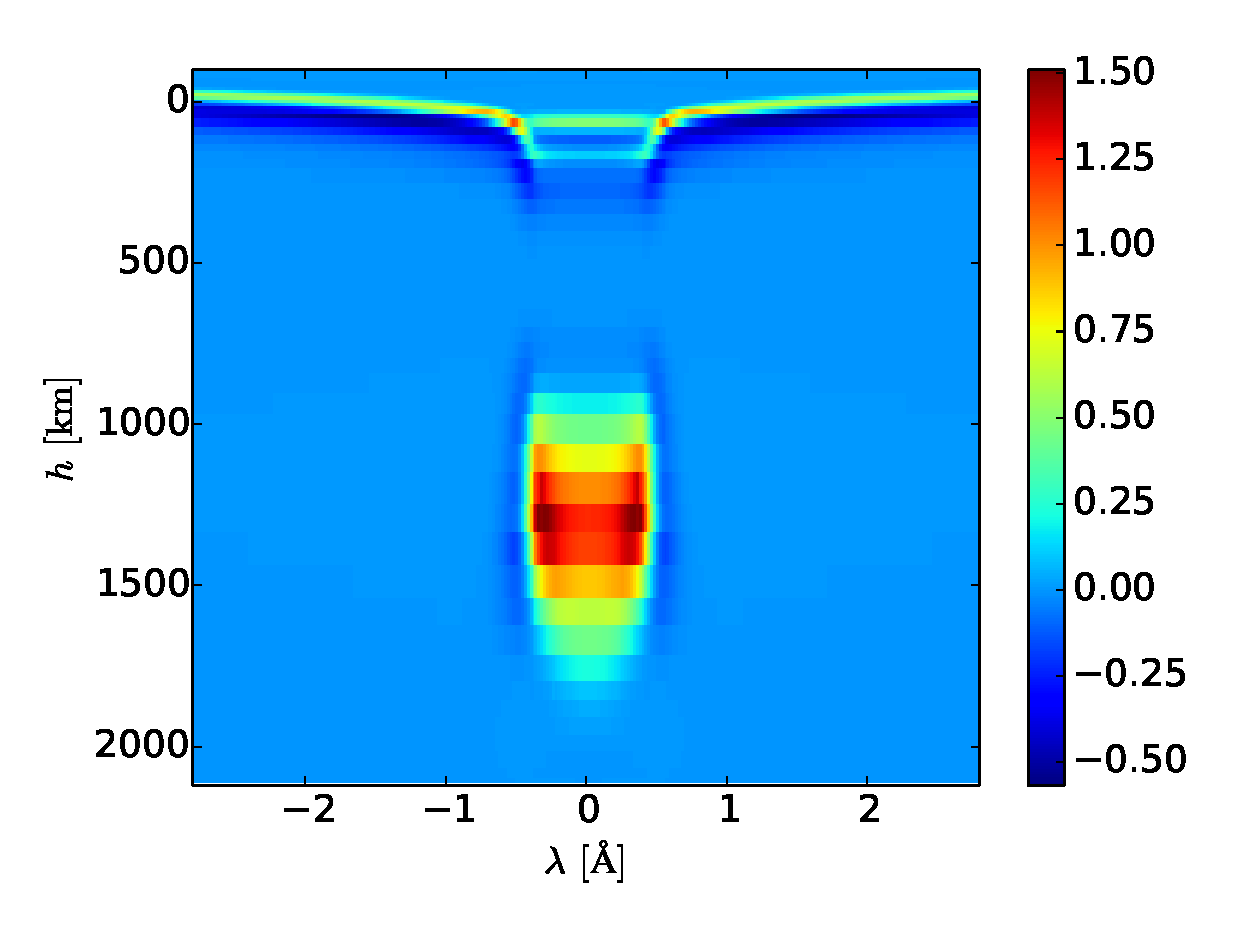
\includegraphics[width = 0.5\textwidth]{ex_1_numerical_responses_intensity_temperature.eps}
 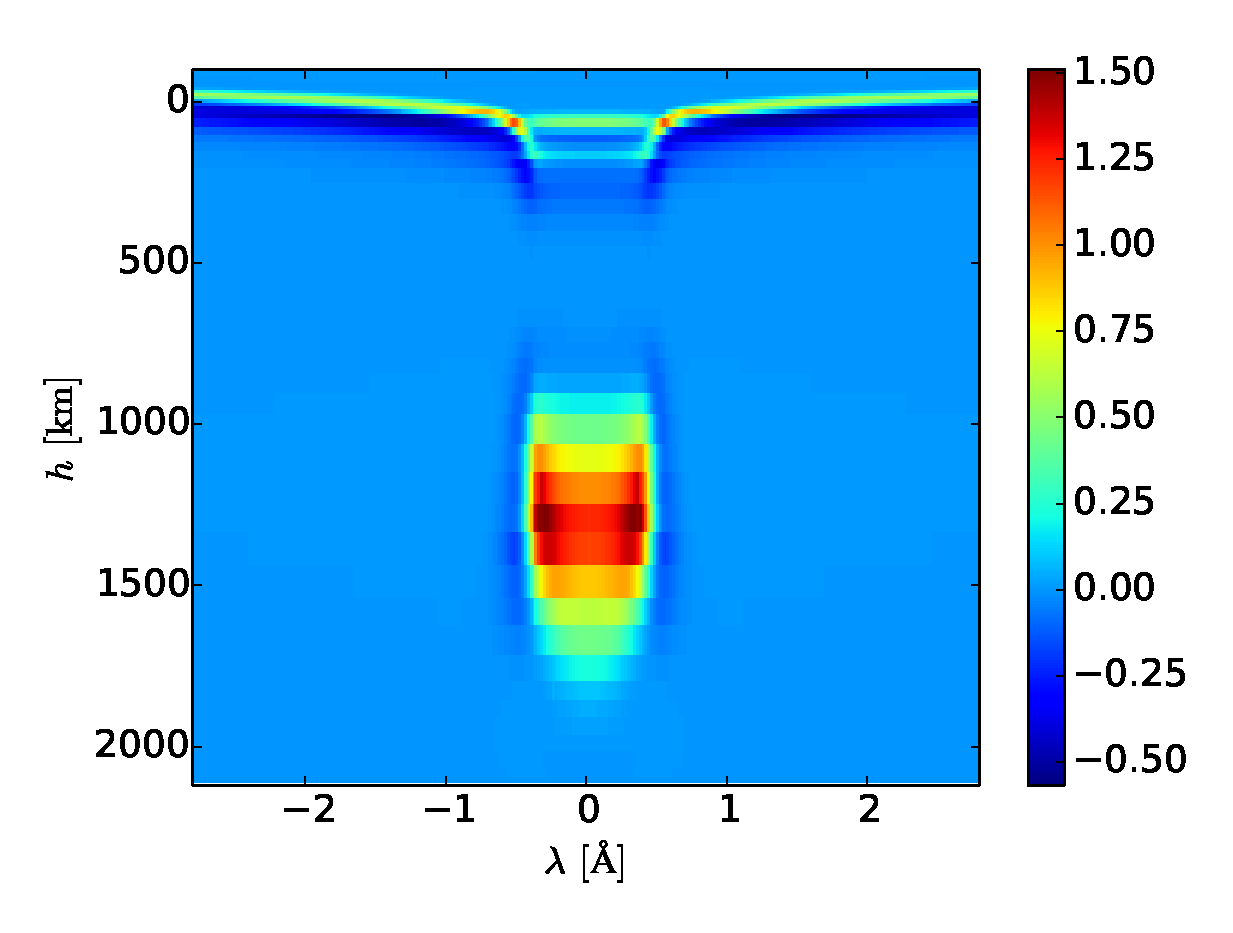
\includegraphics[width = 0.5\textwidth]{ex_1_analytical_responses_intensity_temperature.eps}
 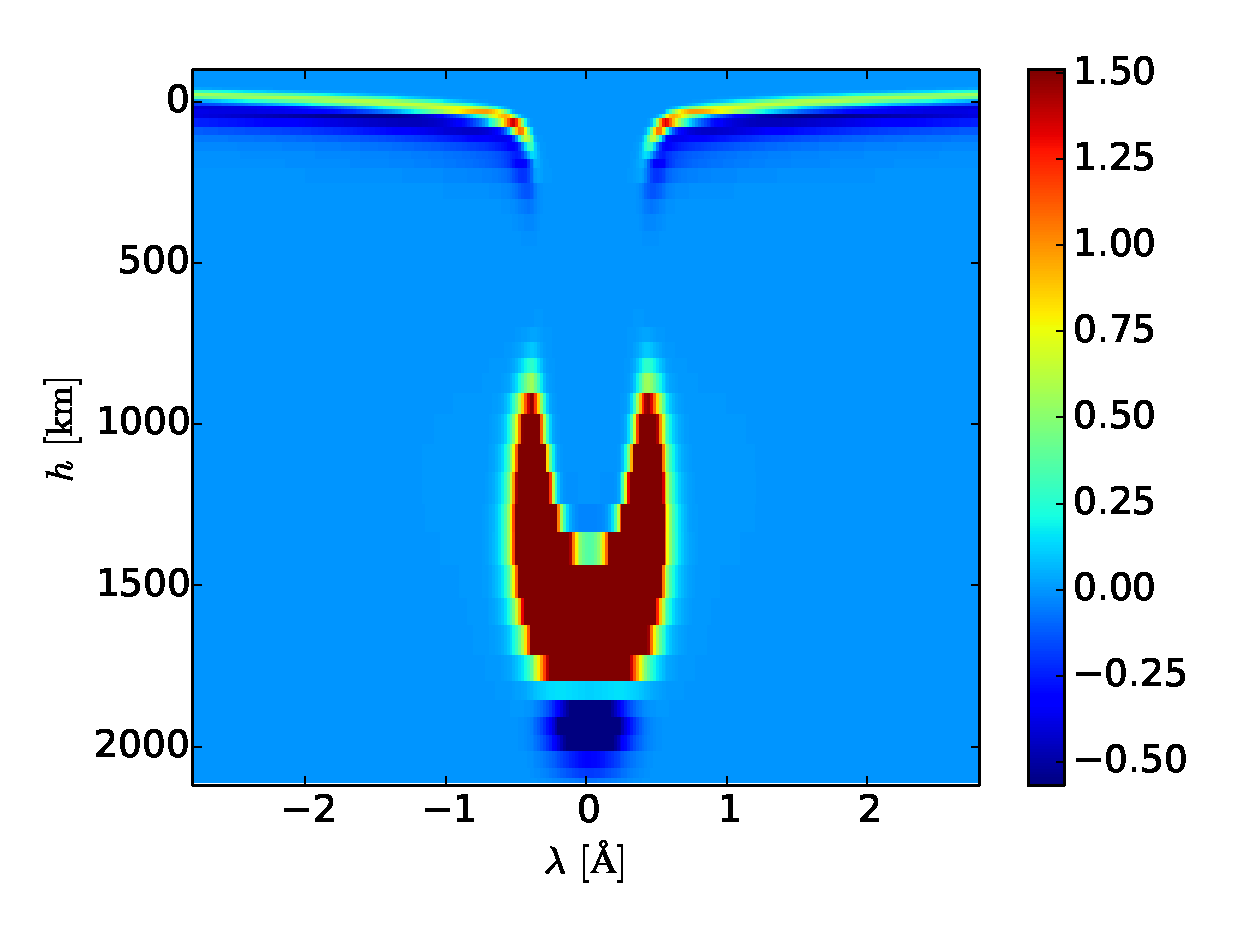
\includegraphics[width = 0.5\textwidth]{ex_1_fdc_analytical_responses_intensity_temperature.eps}
 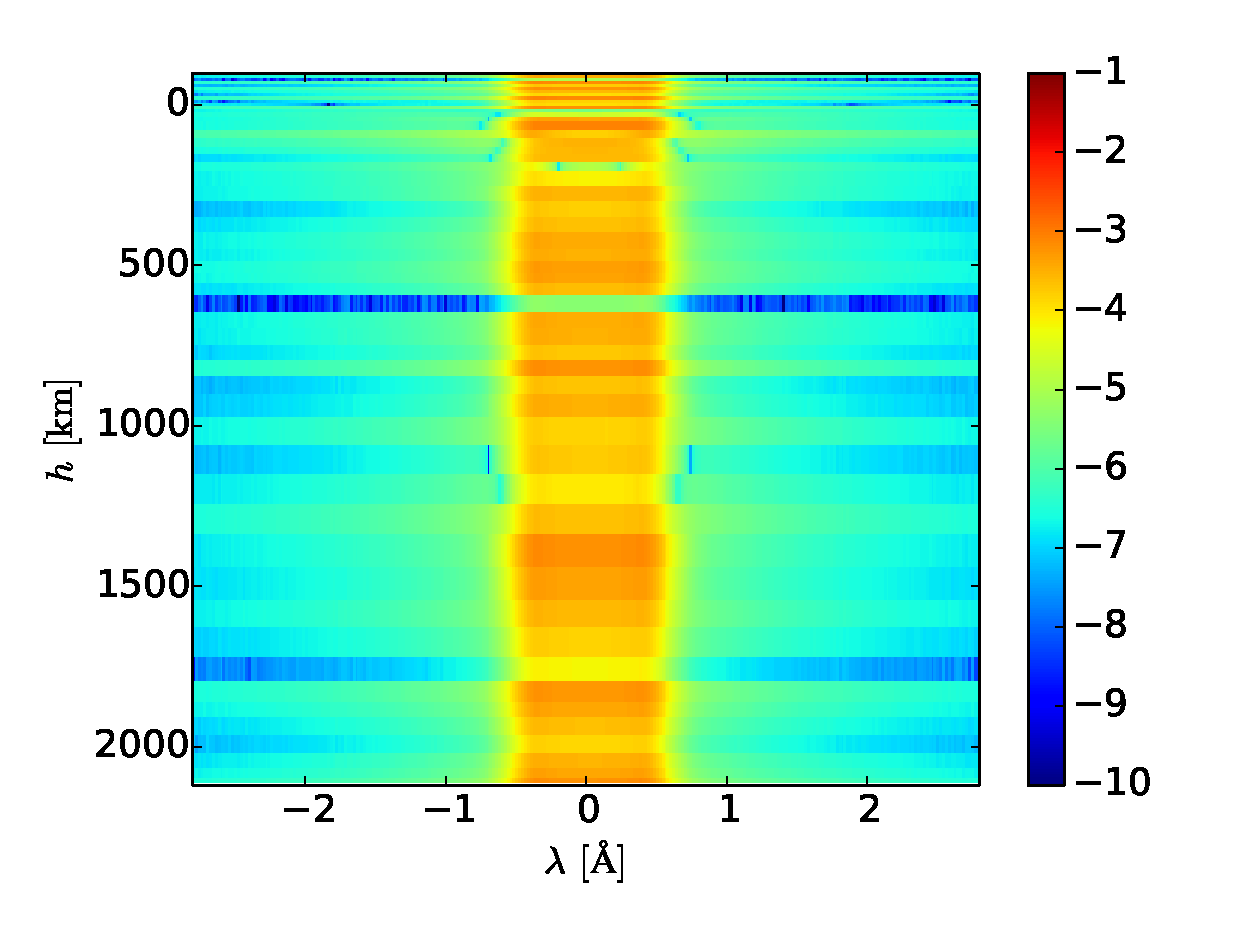
\includegraphics[width = 0.5\textwidth]{ex_1_relative_difference_responses_intensity_temperature.eps}
 \caption{Intensity response functions to temperature for a two-level atom line in FALC model atmosphere normalized with respect to the emergent profile, given in units of $10^{-4}$. Top left: Numerical (finite difference) computation of intensity responses; Top right: Responses computed analytically using the method described in the paper; Bottom left: Responses computed using FDC approach; Bottom right: Relative differences, normalized with respect to the maximum response,  between analytical and numerical computations (in log scale).}
 \label{example_1}
 \end{figure*}
 
The response functions to temperature, computed using the three different approaches are shown in Fig.\,\ref{example_1}. For the numerical computation we have used a perturbation of $1\,\rm{K}$ and converged the NLTE problem down to the greatest relative change in populations of $10^{-8}$. 

The line intensity response functions resemble those computed by \citet{Hector_halpha} (note that the authors there are plotting absolute, normalized response functions, so negative response cannot be seen). We see that the FDC approximation (bottom left) severely overestimates the response to temperature at heights around 1500\,km. The reason for this is that these are computed using the same assumptions as for LTE response functions, that is, the populations respond strictly locally and the response is governed by Saha-Boltzmann statistics. In extreme examples of NLTE lines (such as H$\alpha$), this is a very bad approximation as the level populations are predominantly determined by the radiation field coming from lower layers. It can be seen that response function computed analytically using the method described above (top right), is visually indistinguishable from the one computed using finite differences. The bottom-right panel of Fig.\,\ref{example_1} shows the difference between the analytical and numerically computed response functions, divided by maximum absolute value of the numerical response function, that is:
\begin{equation}
r(h,\lambda) = \frac{\bar{R}^{\rm num}(h_k,\lambda) - \bar{R}^{\rm an}(h_k,\lambda)}{\rm max (|\bar{R}^{\rm num}(h_k,\lambda)|)}.
\end{equation}
$r(h,\lambda)$ is of the order of $0.001\,(0.1\%)$ everywhere in the atmosphere, both for this example and the two considered below. This is a level of agreement which suggest that the analytical response functions describe the line formation process not only qualitatively, but also quantitatively with sufficient accuracy to make use of them in an inversion code. 

 The time needed to set up, compute and de-compose the matrix on the left hand side of Eq.\,\ref{final_linear_system} is, in our specific implementation and for this specific example, smaller then one full NLTE solution, whereas for a model described with $N_P$ parameters, one needs an order of $N_P$ full NLTE solutions to numerically compute the response to all the parameters. Clearly, in this case, the use of analytically computed response functions reduces the computing time significantly.


\subsubsection{Multilevel atom}
We, very briefly present some results obtained using a 4-level hydrogen-like atom. The atom consists of a ground level which is assumed to be in LTE and 3 NLTE levels with atomic constants corresponding to leves 2-4 of hydrogen. As before, we only consider line processes, the difference with respect to the previous example is thus only that the effects of non-linearity are now more pronounced, as we are dealing with a multilevel atom. Fig.\,\ref{example_2} shows the response function of the H$\beta$ line, computed as in the previous example, with a similar level of agreement everywhere in the $(\lambda,h)$ plane.

\begin{figure*}
 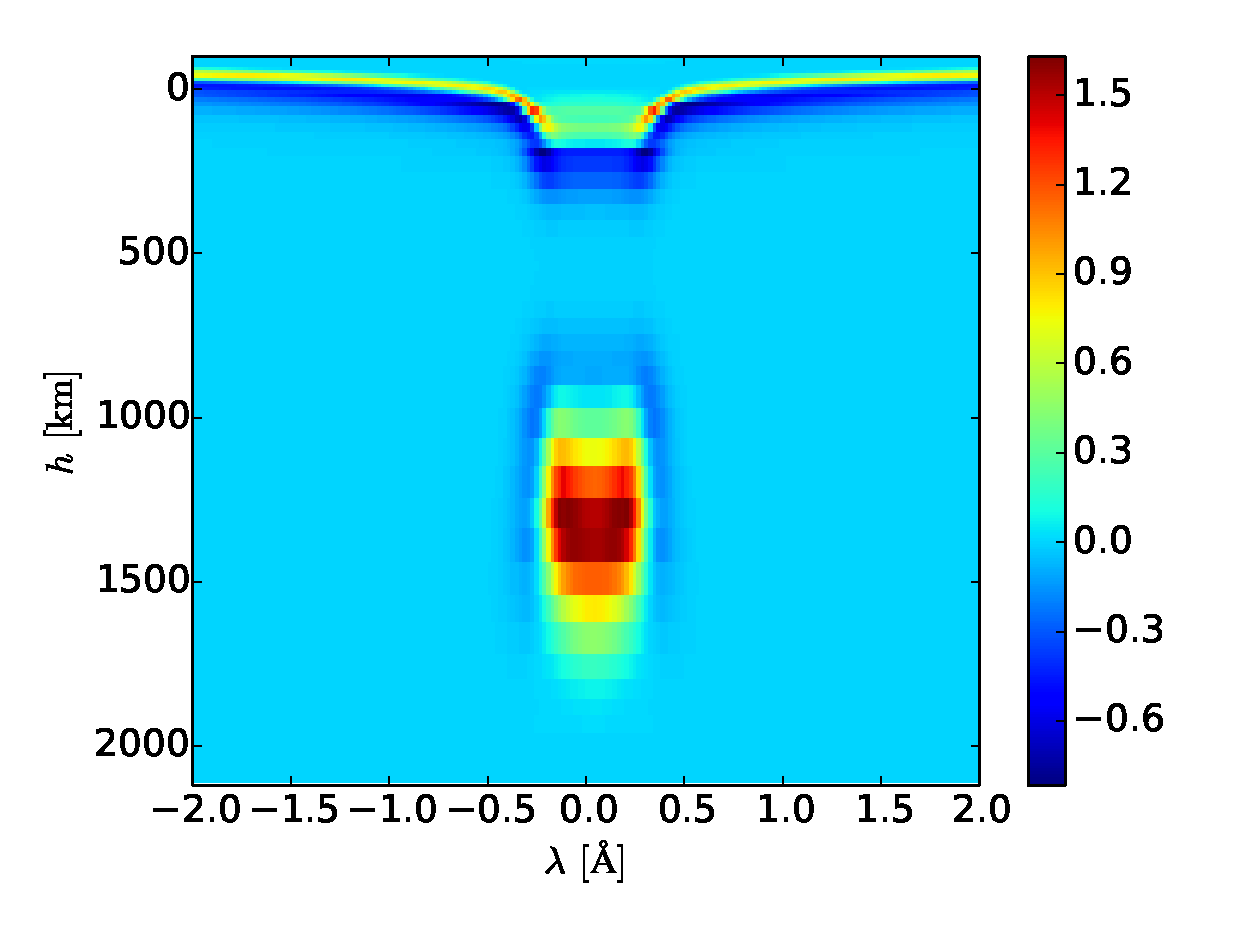
\includegraphics[width = 0.33\textwidth]{ex_2_numerical_responses_intensity_temperature.eps}
 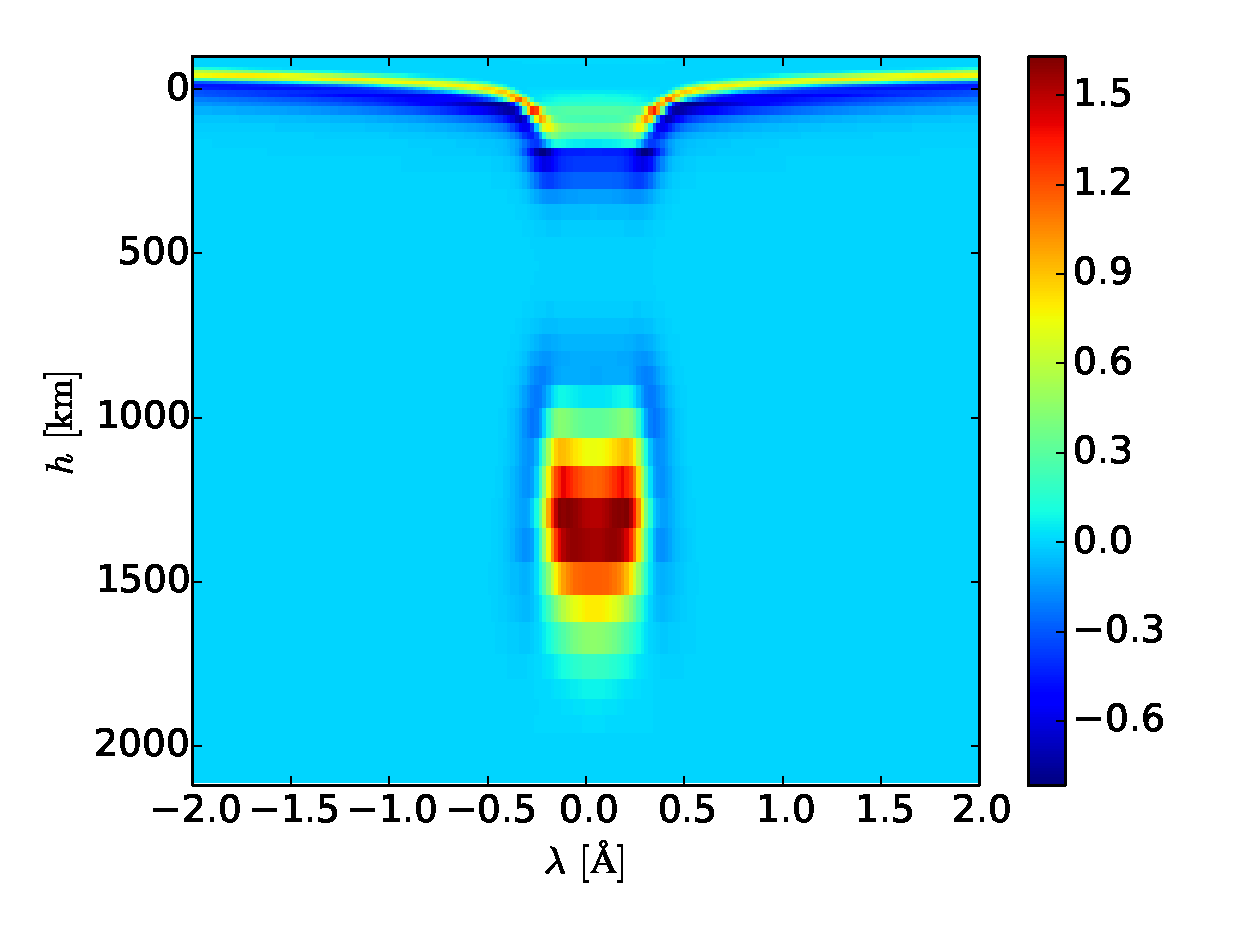
\includegraphics[width = 0.33\textwidth]{ex_2_analytical_responses_intensity_temperature.eps}
 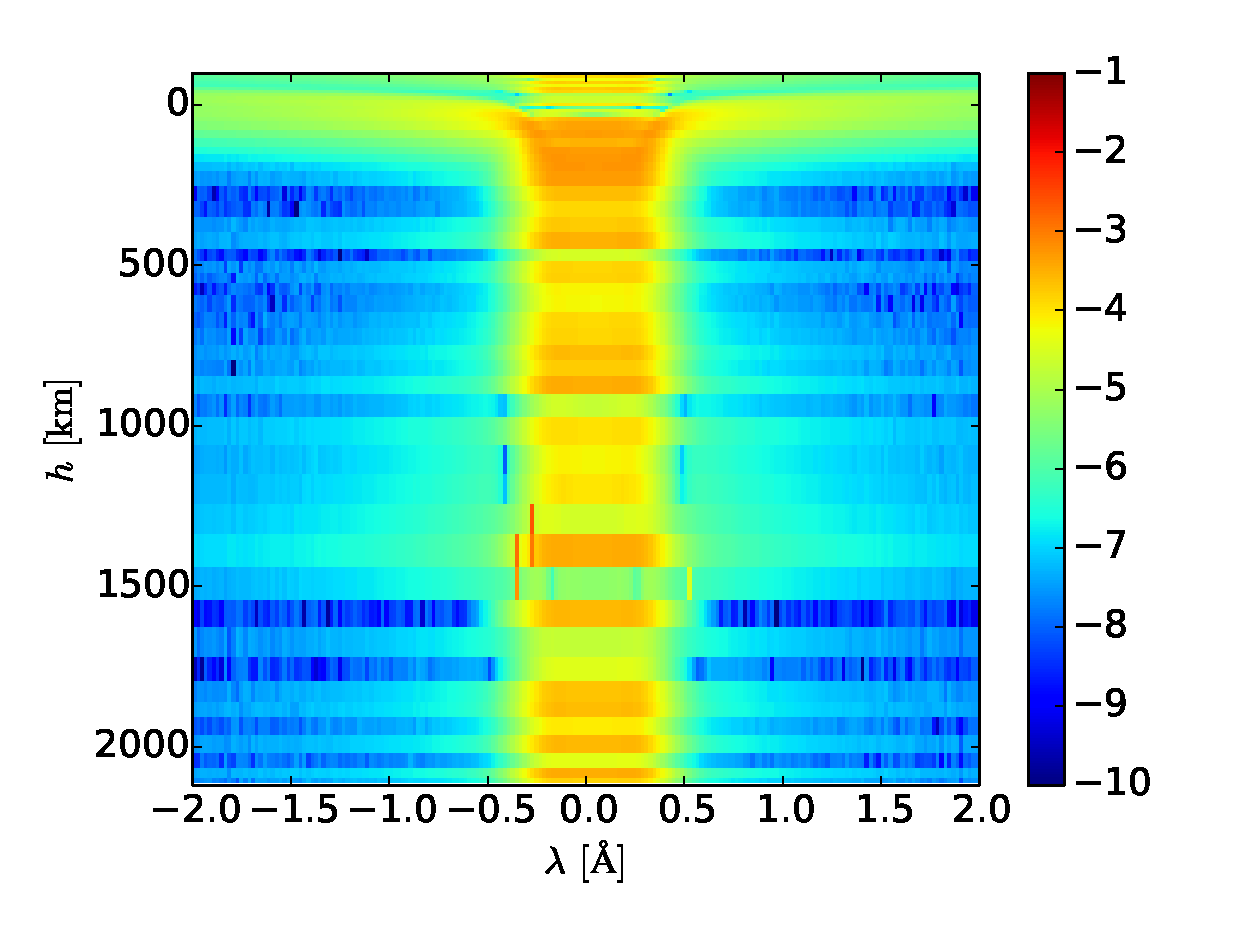
\includegraphics[width = 0.33\textwidth]{ex_2_relative_difference_responses_intensity_temperature.eps}
 \caption{Comparison between numerically (left) and analytically (middle) computed response functions to temperature for emergent intensity in H$\beta$ line, normalized with respect to emergent intensity, in units of $10^{-4}$. Right: absolute difference between the analytical and numerical approach, normalized with respect to the maximum response.}
 \label{example_2}
\end{figure*}

\subsection{The Calcium II 8542 line}
\label{CaII}

The infrared triplet of singly ionized Calcium around 850\,nm are among the most promising candidates for obtaining atmospheric diagnostics \citep[see][for an in depth discussion of response function and diagnostic capabilities]{Ca_diag_Jaime} in the solar chromosphere. The most frequently used member of this triplet, the line at 8542\,\aa, is one of the lines that is routinely inverted using the NLTE inversion code NICOLE, but the numerical cost of calculating the response functions makes such inversions very costly, a situation that has resulted in some authors resorting to approximate approaches \citep{Beck_inversion_2015}. We thus investigate the potential of the analytical response functions for use in inversion codes.

We consider a FALC atmospheric model, without magnetic fields or velocities, and consider a CaII atomic model with 5-levels, as in \citet{Ca_diag_Jaime}. For simplicity, we do not consider line asymmetry due to the presence of isotopes, but this effect should be straightforward to include. Although we now also consider other sources of opacity, namely: H- bound-free and free-free opacity, electron scattering, Rayleigh scattering on neutral hydrogen, and bound-free opacity of the CaII atom, we simplify the problem somewhat by considering the electron density to be in LTE. 

As discussed in \ref{radiative_rates}, we need to take into account all the processes which contribute to the radiative rates, but also to the opacity and emissivity. This means that Eq.\,\ref{derI_inconcise} has to be modified to account for continuum processes. By accounting carefully for the sources of opacity and emissivity and their derivatives, both the LHS, which describes the coupling between all levels at all points in the atmosphere, and the RHS of Eq.\,\ref{final_linear_system} can be appropriately modified and the level responses can be obtained. This process is laborious but straightforward, after which the corresponding opacity and emissivity responses are readily computed and propagated to yield the response of the emergent intensity.

\begin{figure*}
 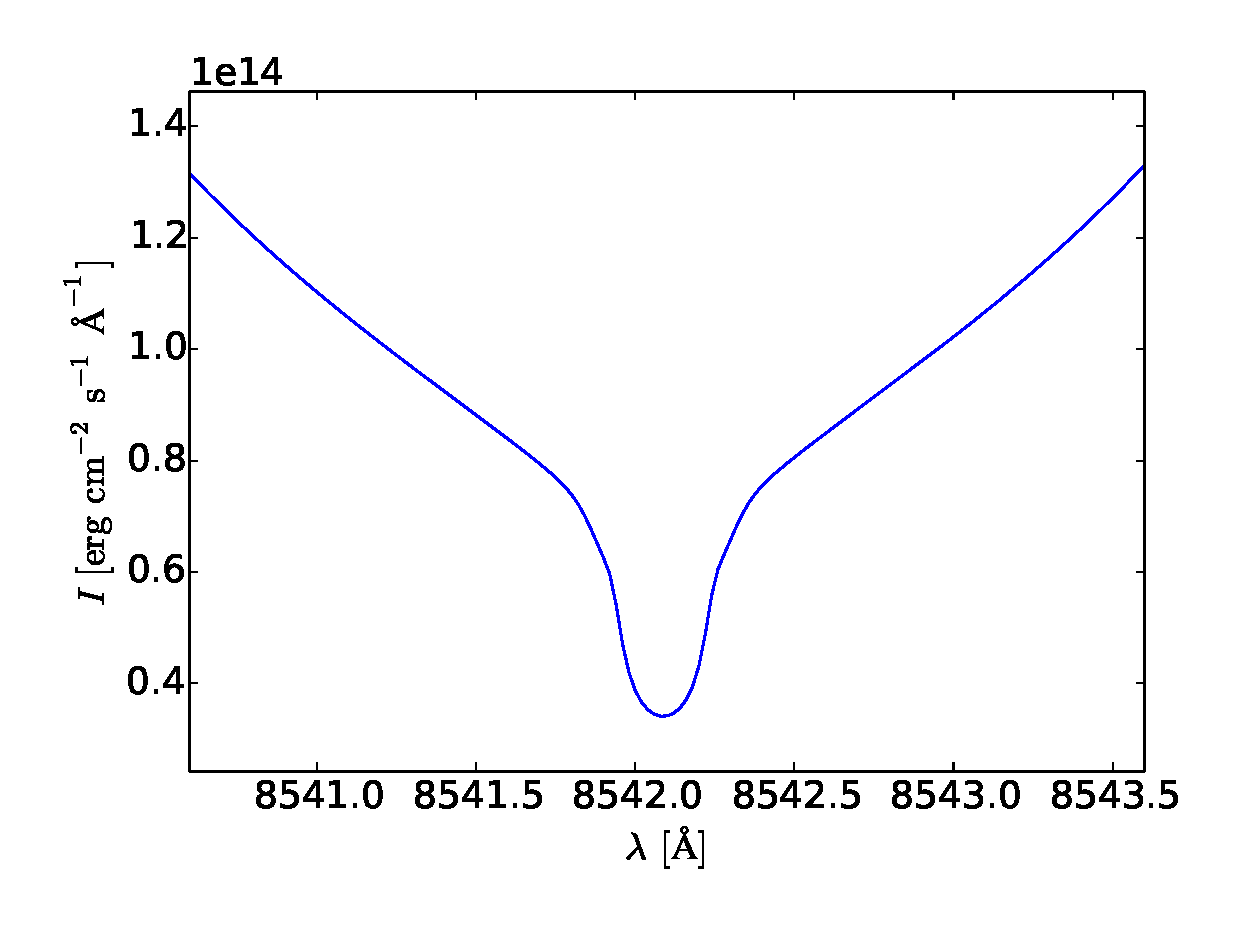
\includegraphics[width = 0.5\textwidth]{ex_3_spectrum.eps}
 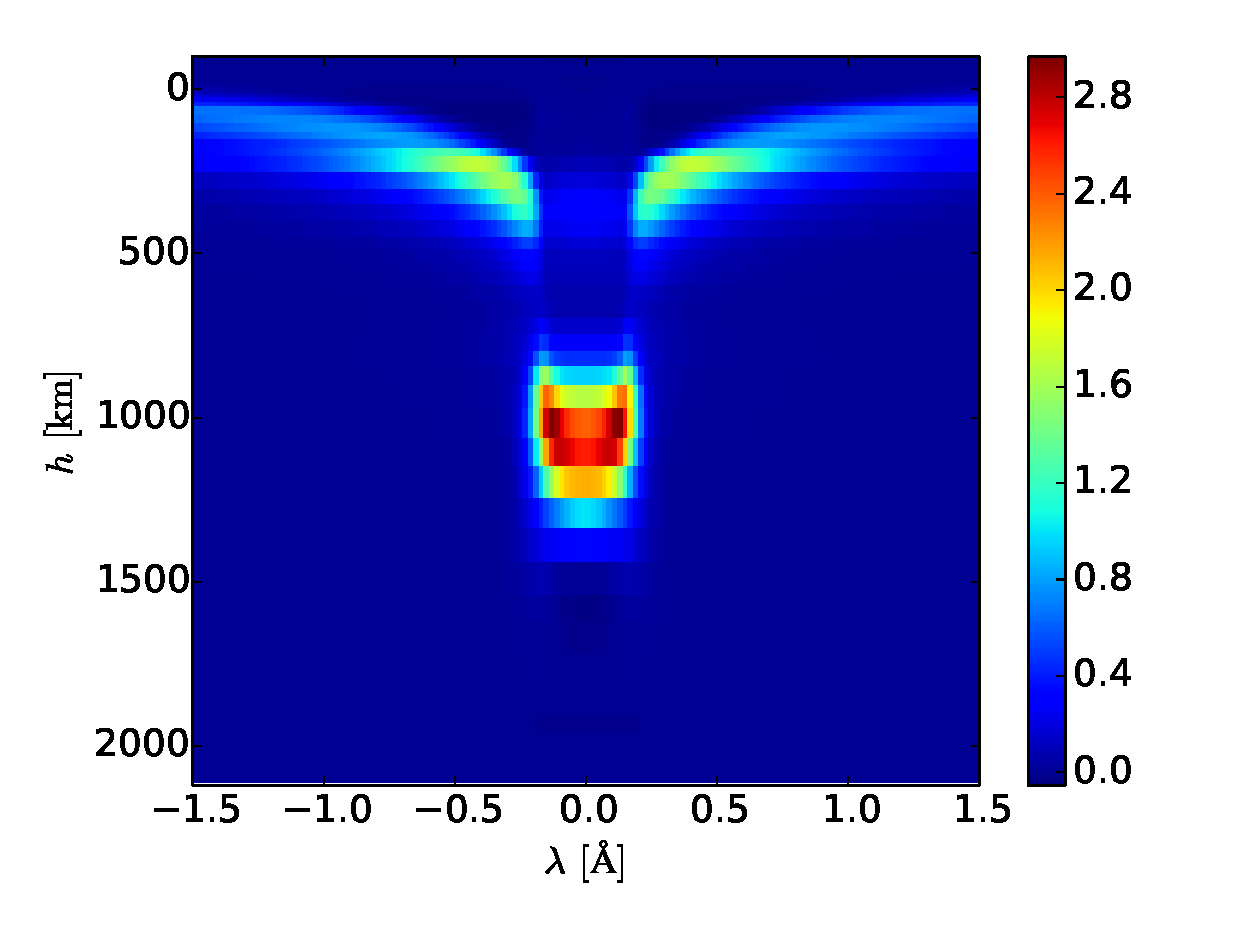
\includegraphics[width = 0.5\textwidth]{ex_3_numerical_responses_intensity_temperature.eps}
 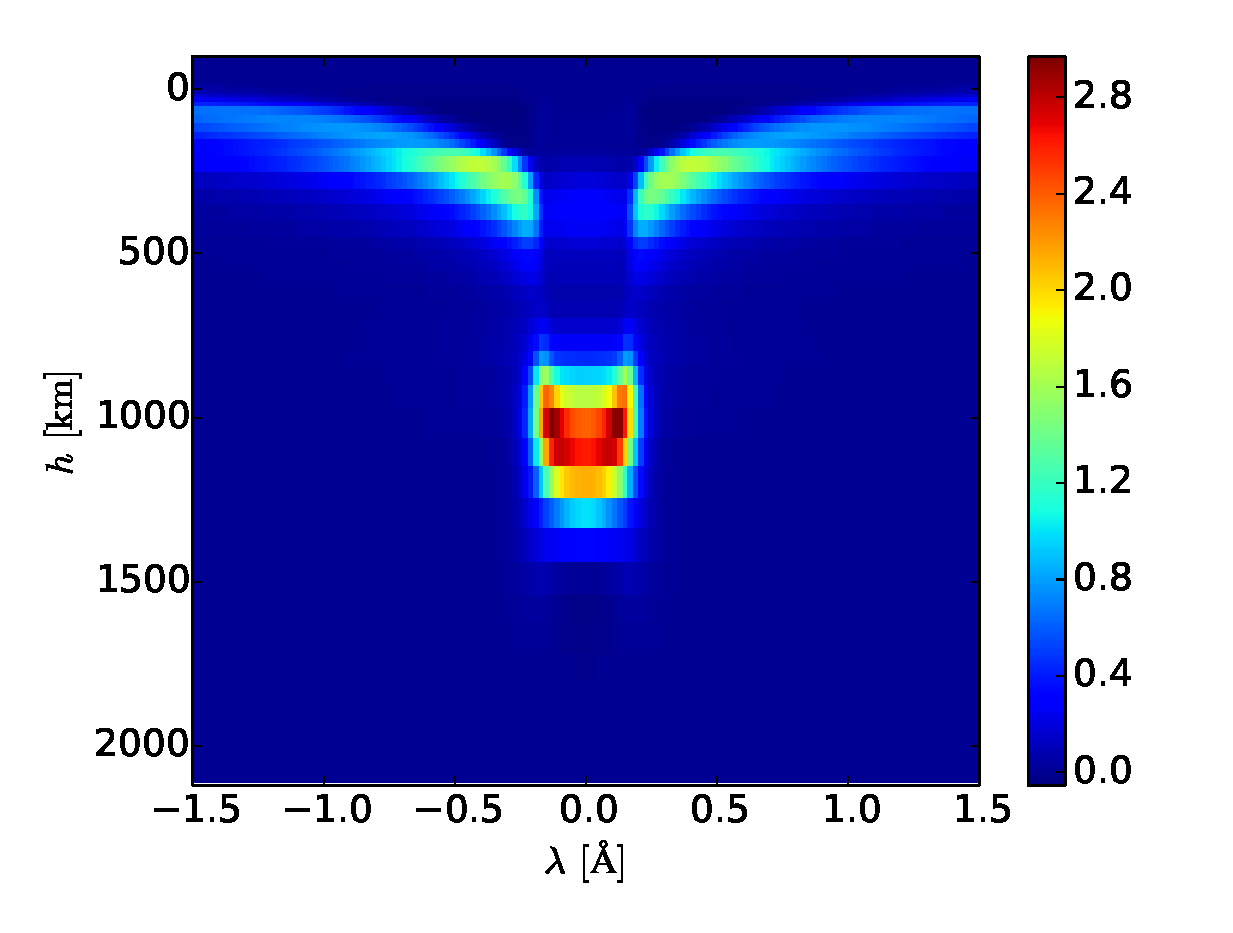
\includegraphics[width = 0.5\textwidth]{ex_3_analytical_responses_intensity_temperature.eps}
 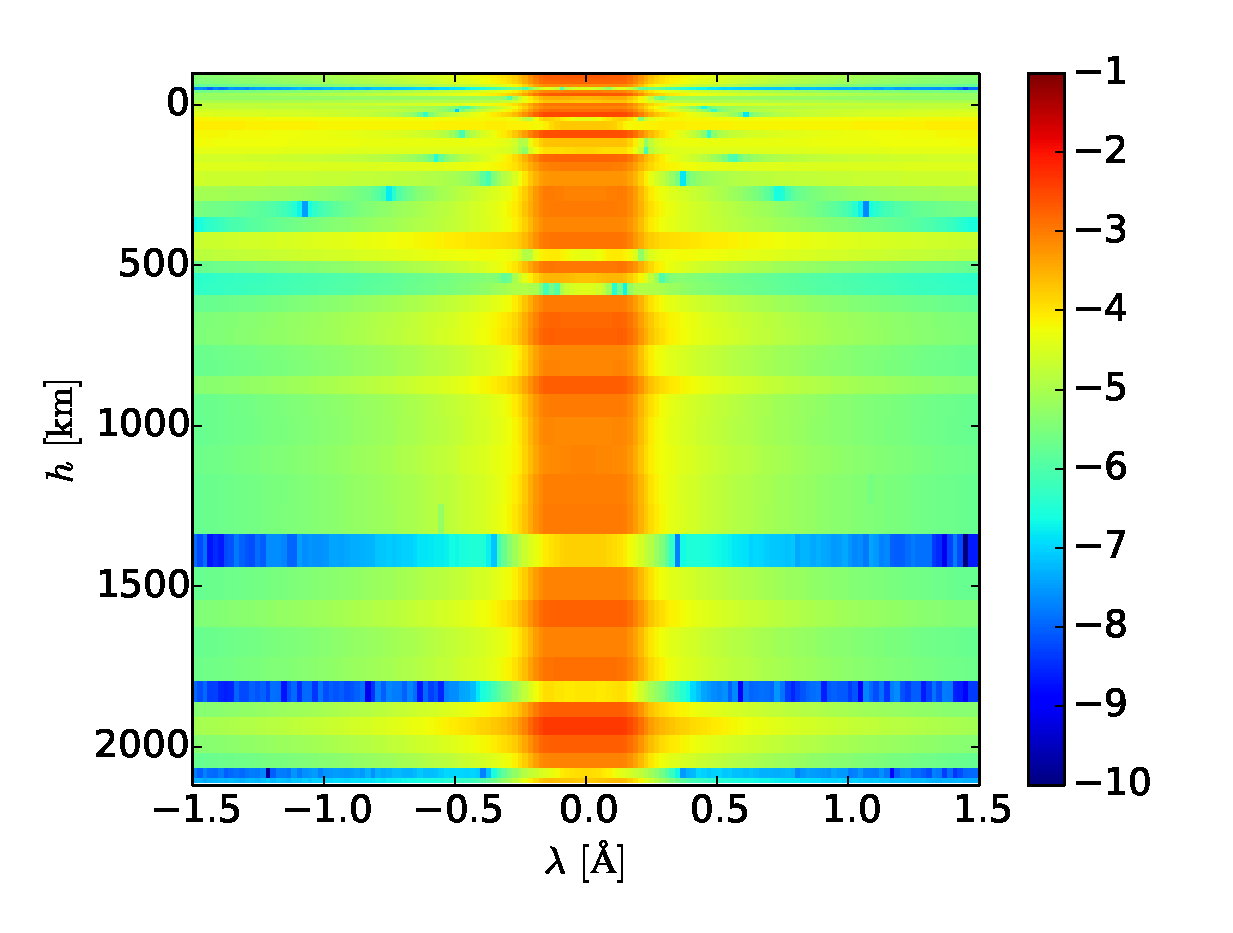
\includegraphics[width = 0.5\textwidth]{ex_3_relative_difference_responses_intensity_temperature.eps}
 \caption{Intensity response functions to temperature for a 8542 Ca line in FALC model atmosphere, normalized with respect to the emergent profile, given in units of $10^{-4}$. Top left: Emergent line profile; Top right: Numerical (finite difference) computation of intensity responses; Bottom left: Responses computed analytically using the method explained in the paper; Bottom right: Absolute differences between analytical and numerical computations normalized to the maximum response (log scale).}
 \label{example_3}
 \end{figure*}

Fig.\,\ref{example_3} shows the emergent line profile and response function to the temperature, computed with finite differencing and analytically. The emergent profile is somewhat different from the one shown in \cite{Ca_diag_Jaime}, which could be due to the absence of magnetic field in our atmospheric model (the metioned authors consider a 500\,Gauss magnetic field), or because of differences in the treatment of the collisional rates. However, this difference is not critical here, as here we are predominantly interested in the response, and not in the accuracy of the physics. We see that the intensity response function computed with the analytical approach and finite-differences are practically indistinguishable, and that their relative differences are fairly small. The response functions are not identical to those in \cite{Ca_diag_Jaime}, in particular, they lack the negative ``dip'' very high in the atmosphere (see their Fig.\,6). However, this feature is not present in the response functions calculated using both methods, and thus points to differences in the atmospheric model, rather than shortcomings in the calculation of the response function itself.

\section{Discussion and Conclusions}

In this paper we have outlined an analytical approach for the computation of the intensity response functions for lines formed in non-local thermodynamic equilibrium (NLTE). We take the derivatives of the rate equations analytically and then follow them through to get a large linear system where the matrix on the LHS describes the coupling between levels and points in the atmosphere (and hence has the dimension of $NL\times ND$) and the RHS describes ``local'' dependencies (e.g. derivatives of the line profile, collisional rates, etc.). The LHS matrix does not depend on the quantity with respect to which the respons is to be calculated, so it can be decomposed once and then used to obtain responses to different model parameters at different depths. Once responses of level populations are known, we use them to compute appropriate responses of opacity and emissivity and then propagate those to get the response of emergent line profile. 

In this paper we have restricted ourselves to the scalar (i.e. polarization-free) case and to the response functions to temperature. We have considered three examples: A pure line transfer example for a 2- and 4-level atom, and a 5 level Ca\,II atom where we focused on the response of Ca\,II\,8542 line. For all the cases considered we obtained excellent agreement between the intensity response function computed using the finite-difference approximation, and the new analytical approach. 

Although a down side of the new method is that all inter-dependencies of the statistical equilibrium must be explicitly taken into account when calculating the derivatives, something that must be carefully checked using finite differences, the advantage of the analytical approach is that it is much faster. For our specific implementation, it takes less time than one NLTE solution, while a finite difference calculation of the same requires ${\mathcal O}(ND)$ NLTE solutions where $ND$ is number of depth points in the atmosphere. 

While this work has its own interesting applications from the standpoint of theoretical radiative transfer, its main intended area of application is that of NLTE inversions. Current state-of-the-art codes use numerical response functions, which are time consuming to calculate, since typically on the order of ten NLTE solutions are needed for one set of derivatives, for each iterative step in minimization procedure. The method presented here would require a computing time similar to that of one NLTE solution and would thus offer an acceleration of one order of magnitude, and a corresponding inversion code is under construction.

%This new method allows straightforward evaluation of the response of radiation anisotropy to the atmospheric parameters which is a first step toward node-based Hanle inversion, which would be a new step in solar spectropolarimetry. 

\begin{acknowledgements}
 We thank Smitha Narayanamurthy and Rafael Manso Sainz for stimulating and useful discussions. 
\end{acknowledgements}

\appendix
\section{Computing intensity responses to opacity and emissivity perturbations}
\label{Appendix_A}

A necessary ingredient in the computation of the response function for the intensity is the computation of the derivative of the specific monochromatic intensity in a given point with respect to opacity and emissivity everywhere in the atmosphere, that is:
$$\frac{\partial I_l}{\partial \chi_l'}$$ 
and 
$$\frac{\partial I_l}{\partial \eta_l'},$$ 
where, for reasons of clarity, we have omitted the dependence on direction and wavelength. The specific intensity depends on the emissivity and the opacity everywhere in the atmosphere, through the radiative transfer equation, which in most cases needs to be solved numerically. Thus, the value of the intensity will depend not only on the opacity and emissivity, but also on the selected numerical scheme. 

It is important to realize that because different radiative transfer solvers yield different results, the use of different solvers will result in different inversion results. We can only try to ensure that our solver is sufficiently accurate for the question at hand and in light of the observational uncertainties.

After adopting a specific formal solver, the task is to compute the response of the intensity in point $l$ to an infinitesimal perturbation of opacity and emissivity in point $l'$. \citet{dtibook} proposed an analytic approach, which, in the scalar case, yields:
\begin{equation}
 \frac{d\delta I}{ds} = -\chi \delta I + \eta_{\rm{eff}},
 \label{a_pert}
\end{equation}
where
\begin{equation}
\eta_{\rm{eff}} = \delta \eta - \delta \chi I
\end{equation}
and quantities with the prefix $\delta$ refer to perturbed quantities. Eq.\,\ref{a_pert} is then solved by a suitable numerical method, typically the same one that was used to solve the radiative transfer equation to obtain the spectrum itself. This approach would be exact if the numerical solution would be infinitely precise. This is, however, not the case, as integrating different functions on a discrete grid yields different inaccuracies. 

An accurate result can be obtained by following the actual process used to obtain the numerical formal solution, and systematically propagating the derivative of each expression through to the end. For this work we use a second order Bezier solver as in \citet{JaimeBezier}, in which the intensity in point $l$ is computed using
\begin{equation}
 I_l = I_{l-1} e^{-\Delta} + w_{l-1}(\Delta)S_{l-1} + w_{l}(\Delta) S_l + w_C(\Delta) C,
 \label{bezier}
\end{equation}
where $\Delta=|\tau_l - \tau_{l-1}|$ and $C$ is the so called control point, which is computed from the derivative of the source function with respect to the optical depth. 

For two given arrays containing the values of $\chi$ and $\eta$ for a particular direction and wavelength, it is necessary to first compute the optical depth scale, source function, and source function derivative with respect to the optical depth, before the Bezier solver can be employed. The computation of the responses of the intensity with respect to the opacity and the emissivity has a few additional steps and requires the derivatives of all quantities in Eq.\,\ref{bezier} with respect to the opacity and the emissivity. The process consists of the following steps:
\begin{enumerate}
 \item Given the opacity, numerically compute its spatial derivative, needed to perform the spatial integration of the opacity, i.e. to get the optical depth.
 \item Compute the response of the opacity derivative to unit perturbations in the opacity at each point.
 \item From the values of the opacity and the spatial opacity derivative, compute the optical depth scale. 
 \item From the perturbations of the opacity and the perturbations of the opacity derivative, compute the perturbations of the optical depth scale. 
 \item From the emissivity and the opacity, compute the source function ($S$) and the perturbations to the source function.
 \item From the values of the source function, compute the derivative of the source function with respect to the optical depth scale ($dS/d\tau$).
 \item From the perturbations of the source function and the perturbations of the optical depth, compute the perturbations of the derivative of the source function.
 \item Using $S$ and $dS/d\tau$, following the Bezier scheme, formally solve the radiative transfer equation to obtain the specific monochromatic intensity at each point in the atmosphere.
 \item Finally, using the responses of $S$ and $dS/d\tau$, compute the response of the intensity at each point in the atmosphere to perturbations in the opacity and the emissivity in each point of the atmosphere. 
\end{enumerate}

The above procedure is cumbersome, especially once translated into actual equations, but straightforward, and it yields the responses ($\partial I_{l}/\partial \chi_{l'}$ and $\partial I_{l}/\partial \eta_{l'}$), which agree to those computed using finite differences down to the level of the non-linearity of the solution as exposed by the finite step size of the finite difference approximation. After these are computed, the response of the intensity at any point to any combination of perturbations in the opacity and the emissivity can be found easily through
\begin{equation}
 \delta I_l = \sum_{l'} \left [ \frac{\partial I_l}{\partial \chi_{l'}} \delta \chi_{l'} + \frac{\partial I_l}{\partial \eta_{l'}} \delta \eta_{l'} \right ].
\end{equation}
We use this method both in the construction of the LHS matrix (i.e. when computing level responses), and for propagating opacity and emissivity perturbations, once the level perturbations are known. This method provides very precise response functions in the LTE case as well (in the case of LTE, level responses can be found immediately), and it is quite possible that it will enable better converging inversion schemes for LTE as well.


\bibliographystyle{aa}  % A&A bibliography style file (aa.bst)
\bibliography{responses} % your references in file: Yourfile.bib


\end{document}
